\section{Referencia de la Clase FPago\-View}
\label{classFPagoView}\index{FPagoView@{FPagoView}}
Muestra y administra la ventana de formas de pago.  


{\tt \#include $<$fpagoview.h$>$}

Diagrama de colaboraci\'{o}n para FPago\-View:\begin{figure}[H]
\begin{center}
\leavevmode
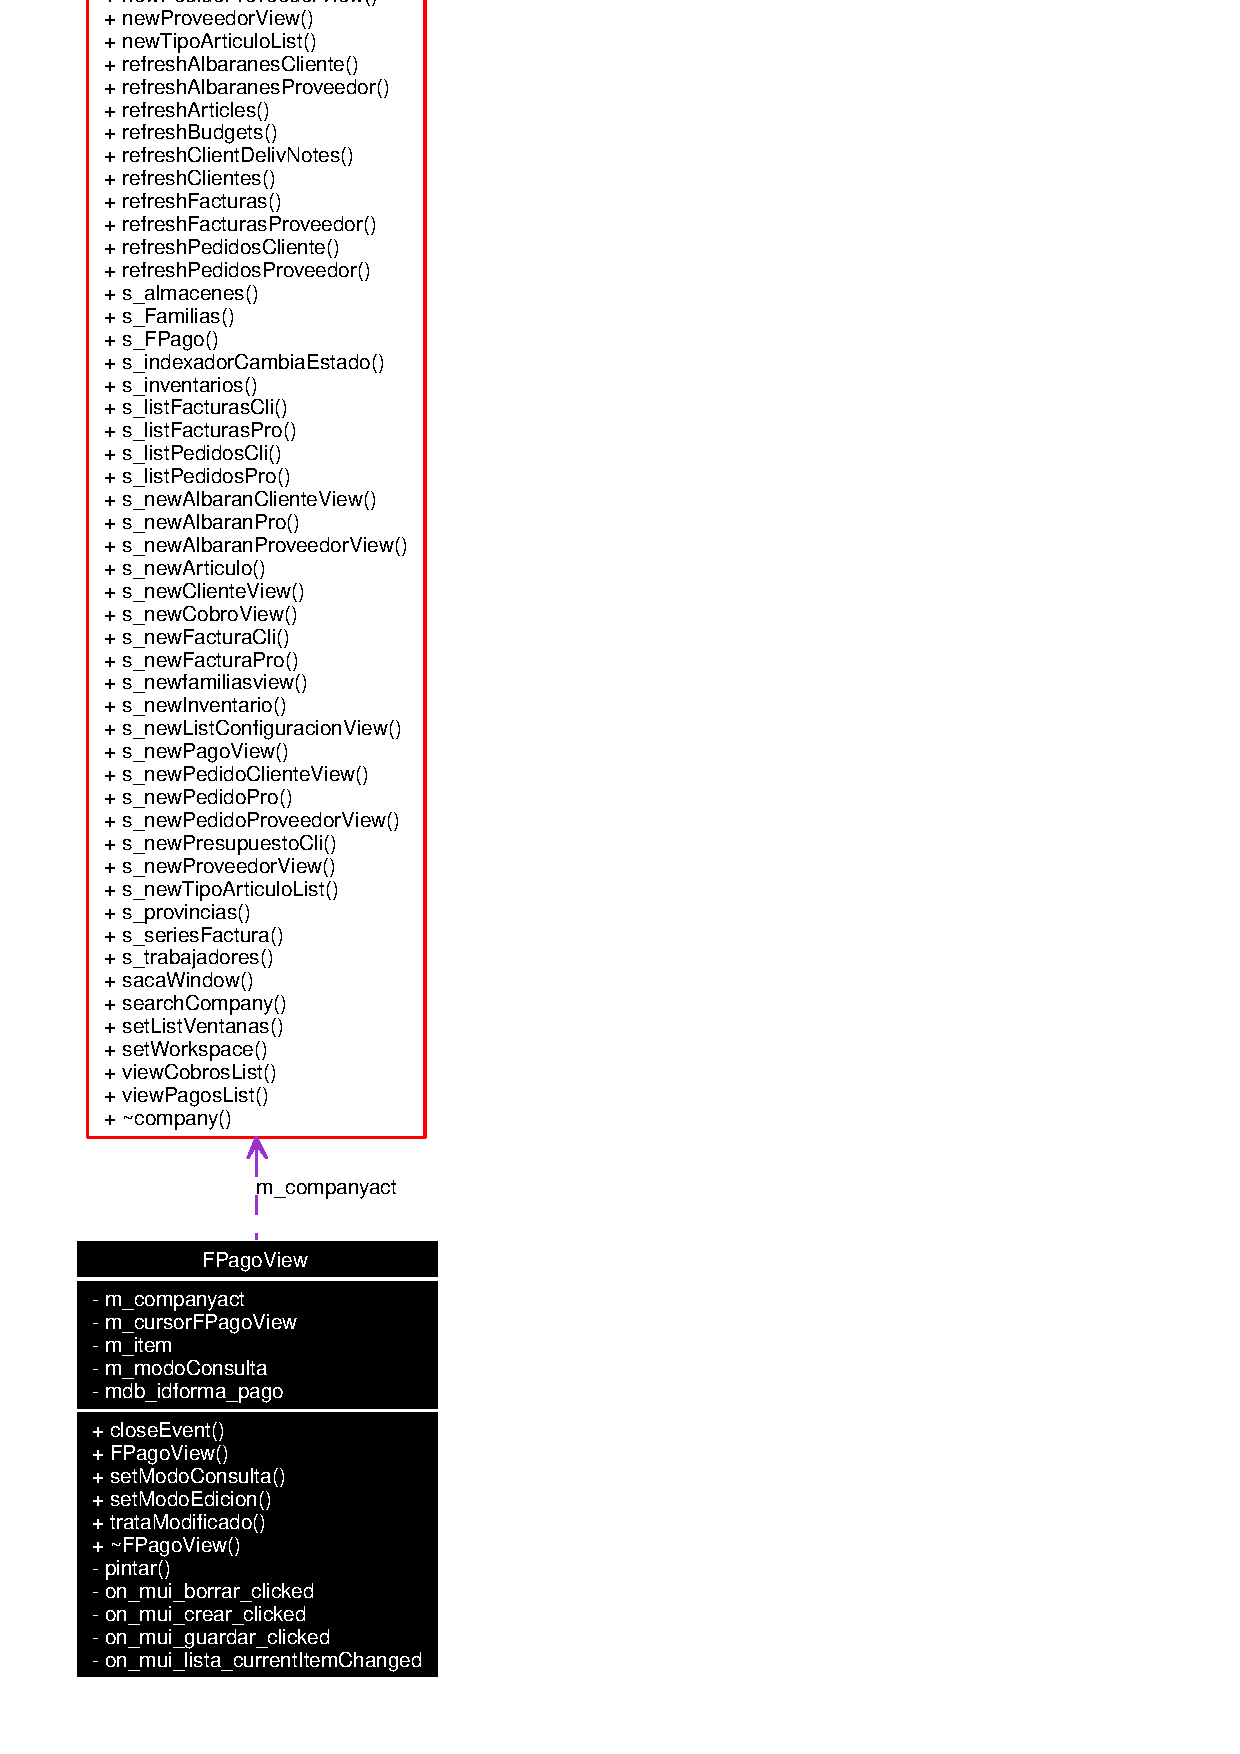
\includegraphics[width=105pt]{classFPagoView__coll__graph}
\end{center}
\end{figure}
\subsection*{M\'{e}todos p\'{u}blicos}
\begin{CompactItemize}
\item 
virtual void {\bf close\-Event} (QClose\-Event $\ast$)\label{classFPagoView_a0}

\item 
{\bf FPago\-View} ({\bf company} $\ast$emp, QWidget $\ast$parent=0)\label{classFPagoView_a1}

\begin{CompactList}\small\item\em Constructor de la clase inicializa la clase y llama a la clase de pintar para que pinte. \item\end{CompactList}\item 
void {\bf set\-Modo\-Consulta} ()\label{classFPagoView_a2}

\item 
void {\bf set\-Modo\-Edicion} ()\label{classFPagoView_a3}

\item 
bool {\bf trata\-Modificado} ()
\end{CompactItemize}


\subsection{Descripci\'{o}n detallada}
Muestra y administra la ventana de formas de pago. 



\subsection{Documentaci\'{o}n de las funciones miembro}
\index{FPagoView@{FPago\-View}!trataModificado@{trataModificado}}
\index{trataModificado@{trataModificado}!FPagoView@{FPago\-View}}
\subsubsection{\setlength{\rightskip}{0pt plus 5cm}bool FPago\-View::trata\-Modificado ()}\label{classFPagoView_a4}


Si se ha modificado el contenido advertimos y guardamos. 

La documentaci\'{o}n para esta clase fu\'{e} generada a partir de los siguientes archivos:\begin{CompactItemize}
\item 
fpagoview.h\item 
fpagoview.cpp\end{CompactItemize}
